%%%%%%%%%%%%%%%%%%%%%%%%%%%%%%%%%%%%%%%%%%%%%%%%%%%%%%%%%%%%%%%%%%%%%%%%%%%%%%%%
%2345678901234567890123456789012345678901234567890123456789012345678901234567890
%        1         2         3         4         5         6         7         8

\documentclass[letterpaper, 10 pt, conference]{ieeeconf}  % Comment this line out if you need a4paper

%\documentclass[a4paper, 10pt, conference]{ieeeconf}      % Use this line for a4 paper

\IEEEoverridecommandlockouts                              % This command is only needed if 
                                                          % you want to use the \thanks command

\newcommand{\ub}{\bar{u}}
\newcommand{\yb}{\bar{y}}
\newcommand{\wb}{\bar{w}}
\newcommand{\Hc}{\mathcal{H}}

\overrideIEEEmargins       
\usepackage{todonotes}                              
\RequirePackage{graphicx}
\graphicspath{ {figures/} }
% See the \addtolength command later in the file to balance the column lengths
% on the last page of the document

% The following packages can be found on http:\\www.ctan.org
%\usepackage{graphics} % for pdf, bitmapped graphics files
%\usepackage{epsfig} % for postscript graphics files
%\usepackage{mathptmx} % assumes new font selection scheme installed
%\usepackage{times} % assumes new font selection scheme installed
%\usepackage{amsmath} % assumes amsmath package installed
%\usepackage{amssymb}  % assumes amsmath package installed

\title{\LARGE \bf
Heart-on-a-Chip platform for closed-loop testing of cardiac devices
}

\author{Albert Author$^{1}$ and Bernard D. Researcher$^{1}$% <-this % stops a space
\thanks{*This work was partially supported by ???}% <-this % stops a space
\thanks{$^{1}$The Electrical and Systems Engineering Department, University of Pennsylvania, Philadelphia, U.S.A.
        {\tt\small \{habbas,zhihaoj,rahulm\}@seas.upenn.edu}}%
}


\begin{document}

\maketitle
\thispagestyle{empty}
\pagestyle{empty}


%%%%%%%%%%%%%%%%%%%%%%%%%%%%%%%%%%%%%%%%%%%%%%%%%%%%%%%%%%%%%%%%%%%%%%%%%%%%%%%%
\begin{abstract}
This paper proposes a closed-loop testing setup for pacemakers, in which the pacemaker is connected to a Virtual Heart Model (VHM) and both device and heart signals are used to assess correctness of the device's operation. 
The test inputs are automatically generated by a requirements-guided algorithm that uses the desired heart behavior as a guide for finding test cases that violate it.
These can be replayed by the designer to determine whether the pacemaker operated incorrectly.
The advantages of closed-loop testing over open-loop testing are illustrated with two experiments involving the VHM and a validated pacemaker model.
\end{abstract}
\section{outline}

Intro:\\
- The human heart: a normal EKG, examples of arrythmias.
\\
- Stress that the interpretation of EKGs is complex and equal parts art and science.
\\
- Pacemakers: what is their function, how they are developed
\\
How pacemakers are developed today: code modules, rule-based

Two main decisions when testing:\\
- what input sequences to provide\\
- how to determine correctness of output\\
Ideally:\\
- the input sequences to the device are those that will be generated by heart reacting to the PM's outputs.
\\
- the device correctness is determined by looking at the heart's behavior: is it safe? Safety is a domain-specific concept and must be determined by the physician.

Important: if the heart displays unsafe or undesired behavior, then this means there's room for improvement, but not that the PM should be thrown out. Depending on what our constraints are, some undesired behavior might have to be tolerated if it is a consequence of an even more desirable operation of the PM.

Pacemaker testing today: open-loop. 
Show examples from Medtronic

The shortcomings of open-loop testing:
\\
- only uses input sequences that were thought of by validator, thus might miss inputs provided by the heart and which PM must accommodate. \textbf{how this manifests itslef}: undesired heart behavior even though PM satisfies its spec.
\\
- the measure of correctness is what the PM does, not what the heart does. Going from what we would like the heart to do to what the PM should do is an error-prone, manual, intuitive process.
\textbf{how this manifests itself}: the PM functions correctly (according to its spec) on a heart input that \emph{was} part of the test suite, but the heart does something undesired.
\\
- open-loop tests can still be run in a closed-loop setting via initialization. Only now, we get to see how the heart reacts to the PM and thus determine whether the intended effect is achieved. 


Closed-loop testing connects the heart to the pacemaker. The controlled variables are disturbances like PVC and PAC, and parameters of both pacemaker and heart.
\\
- The input sequences to the PM are provided by the heart, so there's no issue of missing waveforms. we have a systematic way fo exploring the space of inputs (even if we might not get to all of it because of time limitation)
\\
- the correctness is determined by the heart's behavior, as it should.
\\
- can use an actual pacemaker: the HoC 

But we don't have hearts lying around for testing -> heart models.

Specification-guided testing: given the specification that we wish to test, guide the testing process towards behavior that might falsify it, thus producing a concrete counter-example for hte designer to use as feedback.

Experiments:\\
- example of finding a model error \\
- example of undesired behavior

Future:\\
- Enrich the heart model \\
- run on the HoC

\section{Introduction}
\label{introduction}

Medical devices like implantable pacemakers are designed to diagnose and improve undesired physiological conditions. The capability to affect the physiological conditions of the patient makes the safety of the devices an essential consideration. The software component of these devices are getting increasingly complex, inevitably leading to more safety violations. From 1996-2006, the percentage of software-related causes in medical device recalls have grown from 10\% to 21\%~\cite{recalls}. During the first half of 2010, the US Food and Drug Administration (FDA) issued 23 recalls of defective devices, all of which can cause serious adverse health consequences or death. At least six of the recalls were caused by software defects~\cite{killedbycode}. 

To ensure the safety and efficacy of a device software, we first need to ensure that the device software exhibit the input-output relationship as designed, which are captured in the \emph{Software Specifications}. However, we also have to ensure that the device software is capable of improve the physiological conditions as expected, which are captured in the \emph{Physiological Requirements}. The procedure evaluating the conformance between the device software and these two design documents are referred to as \emph{Verification}. The US FDA requires device manufacturers to submit \emph{sufficient evidence} regarding the safety and efficacy of the devices before they can be released to the market. The specifications of the device software is verified using \emph{open-loop testing} in which the devices are given input signals and their outputs are compared with expected outputs according to the design. However, open-loop testing is not effective in finding safety violations which have deeper executions and corresponding to real physiological context. The physiological requirements have to be verified in closed-loop testing in which the devices are tested within its physiological context. Currently the physiological requirements are mostly verified in terms of  \emph{clinical trials} in which the devices are implanted in selected groups of patients and monitored over certain period of time. The limitations of clinical trials are both extreme high cost and limited sample size of patient groups.

Model-based design enables closed-loop verification at earlier design stage. The device (or corresponding software or even mathematical model) interacts with a physiological model which can simulate signals into the device and respond to device outputs. In this work, we use a physiological heart model 


\section{Method: Requirements-guided closed-loop testing}
\label{method}

%\begin{figure}[!t]
%	\centering
%	\includegraphics[scale=0.4]{reqGuidedTesting.pdf}
%	\caption{\small Requirements-guided closed-loop testing methodology.}
%	\label{fig:reqGuidedTesting}
%\end{figure} 
\begin{figure}[!t]
	\centering
	\includegraphics[scale=0.3]{figures/HOCannotated.pdf}		
	\caption{\small Heart-on-a-Chip platform, showing the pacemaker and the microcontroller running the Virtual Heart Model code.}
	\label{fig:hoc}
\end{figure} 

Figure \ref{fig:reqGuidedTesting} shows the requirements-guided closed-loop testing setup that we use in this paper to find unsafe or undesirable behavior of the heart connected to the pacemaker.
In what follows, we describe each component in details.

\input{heartModel}
\subsection{The Heart-on-a-Chip platform}
\label{HoC}

\begin{figure}[!t]
	\centering
	\includegraphics[scale=0.4]{HOCannotated.pdf}		
	\caption{\small Heart-on-a-Chip platform, showing the pacemaker, the microcontroller running the VHM code, and the monitors.}
	\label{fig:hoc}
\end{figure} 
Our closed-loop testing scheme ranges across different stages of the development process. Closed-loop testing can not only be performed on pacemaker models and code, but also on off-the-shelf pacemakers. \figref{hoc} shows the Heart-on-a-Chip (HoC) platform for closed-loop testing of pacemakers. The platform consists of a micro-controller with heart model implemented on it, and an analog interface which convert heart signals
%Before describing the advantages of closed-loop testing, we introduce the Heart-on-a-Chip (HoC) platform, which will be used for the development of closed-loop testers.
%See Fig.~\ref{fig:hoc}.
%\todo[inline]{more...}

\section{Closed-loop Testing of Pacemaker}
\label{closedloop}

= SS: Closed-loop.
Table comparing closed-loop with open-loop.
Robustness-guided testing.
%\subsection{Limitations of Current Practice: Open-loop Testing of Pacemakers}
\label{todaysPractice}
\begin{figure}[tb]
	\centering
	\includegraphics[scale=0.2]{placeHolder.pdf}
	\caption{Setup for pacemaker operation: the device (pacemaker), the plant (human heart), external disturbances (PVCs and PACs), and initial states and parameters (refractory periods, various settings).}
	\label{fig:liveSetup}
\end{figure}
Consider Fig.\ref{fig:liveSetup}, where a typical setup of pacemaker operation is presented.
The Device Under Test (DUT) is connected to the Plant (here, a human heart) which it is meant to control.
Together, they are referred to as the \emph{closed loop}, whereas the DUT alone is an \emph{open loop}.
The plant receives inputs from the DUT, but can also be subject to \emph{external disturbances}: in our case, we consider PVCs and PACs to be external disturbances.
The terminology is meant to convey that these disturbances are inputs to the heart that do not originate in the DUT, but elsewhere. 
The origin of these disturbances need not be modeled.  
They are \emph{disturbances} because they are uncontrolled and can prevent the closed loop from achieving its objectives, namely, a safe and reliable heart operation.

The outputs of the pacemaker are denoted by the letter $u$, e.g. $u = [A_{pace}, V_{pace}]$.
Let $U$ be the set of possible $u$ values.
These constitute inputs to the heart, or plant.
The outputs of the heart are denoted by the letter $y$, e.g. $y = [A_{sense}, V_{sense}]$.
Let $Y$ be the set of possible $y$ values.
These constitute inputs to the pacemaker, or DUT.
A finite sequence, or \emph{string}, of $u$ values will be denoted by $\ub$, and the set of \emph{all} finite $u$-sequences will be denoted by $U^*$: $\ub \in U^*$.
Similarly, we define $\yb \in Y^*$ to be a finite $y$-string.
The disturbances are denoted by $w$, their set of possible values by $W$, and strings of disturbance values by $\wb \in W^*$.

A (discrete-time) \emph{open-loop test} $\yb$ for the DUT is a string $\yb = y_1 y_2 \ldots y_n \in Y^*$.
As a result of being fed a test, the DUT will synchronously produce a string $\ub = u_1 \ldots u_n \in U^*$.
A (discrete-time) \emph{closed-loop test} $\wb$ for the closed loop DUT+Plant (pacemaker + heart) is a string $\wb = w_1 w_2 \ldots w_n \in W^*$.
As a result of being fed a test, the closed loop will synchronously produce a string $(\ub,\yb) \in U^* \times Y^*$.
%The plant $\Hc$ may be seen as an input-output map: $\Hc: U^* \rightarrow Y^*$, where $U^* (Y^*)$ is the set of finite strings over the set $U$ ($Y$).

\subsection{Testing objectives}
\label{testingObjectives}
When testing a pacemaker, or any device in general, two crucial decisions must be made:
\begin{itemize}
	\item Choice of inputs: first, what input strings should be provided to the device so its behavior can be observed in reaction to them? 
	Ideally, the answer is: all input sequences that might be produced by the heart to which the device will be connected. 
	Sequences from outside this set are irrelevant, and missing sequences from within this set might cause us to miss some bugs that will manifest themselves during live operation.
	In what follows, we use $A_\Hc$ to denote the set of strings that might be produced by the heart when connected to the pacemaker in a closed loop as shown in Fig.\ref{fig:liveSetup}. 
	Of course, $A_\Hc \subset Y^*$.
	\item Criterion of correctness: secondly, how do we determine that a particular operation of the device is correct? 
	In other words, what is the specification according to which the device is being tested?
	Ideally, the answer is: the specification will describe the safe, acceptable operation of the heart. 
	I.e. the device is correct if the heart it is controlling does not produce unsafe or undesirable behavior.
	Because the heart is a complex system and its `acceptable' behavior is dependent on its structural characteristics and current condition, such specifications are hard to describe. 
	Nonetheless, this is the standard for what a specification should be for the DUT. 
	A DUT that violates this specification may or may not be modified, depending on the source of the violation. 
	The task of interpreting test outcomes and acting upon them is left to the designer and physician.	
	The validation engineer's task is to produce a trace that violates the specification, or confirm that the DUT does not violate it with high confidence.
\end{itemize}
Note that we distinguish between unsafe heart behavior and undesirable heart behavior: unsafe behavior is not tolerated under any circumstances.\todo[inline]{give example}
Undesirable behavior may not be ideal, but it might be acceptable under certain conditions. 
\todo[inline]{give example}
It is important to understand the circumstances under which undesirable behavior occurs, and then decide whether this is acceptable or not.
In Section \ref{experiments}, we illustrate such a case.
The goal of testing is to establish that the heart's behavior is never unsafe, and establish conditions under which it might be undesirable.

\subsection{Open-loop testing}
\label{openLoopTesting}
\begin{figure}[tb]
	\centering
	\includegraphics[scale=0.2]{placeHolder.pdf}
	\caption{Open loop testing setup: the device (pacemaker) is fed with pre-programmed open-loop tests.}
	\label{fig:OLtestingSetup}
\end{figure}
Today, pacemakers are tested in an open loop \todo[inline]{cite}.
That is, the pacemaker is not connected to the heart, as shown in Fig.\ref{fig:OLtestingSetup}.
Rather, the validation engineer provides the DUT with $N$ open-loop tests
\[A_{OL} = \{\yb_k, k=1,\ldots,N\}\]
E.g., each test is a string of $A_{sense}$ and $V_{sense}$ values. The validator observes the DUT's output $\ub$ to determine correctness.
The tests $\yb_k$ are meant to mimic some possible signals produced by the heart and are designed in consultation with physicians.
They are also \emph{the same tests that were used when designing the pacemaker}.
\todo[inline]{check that last statement}
What the pacemaker's reaction should be is decided based on a diagnosis of the heart signals $\yb_k$:
that is, the physician diagnoses what might cause the heart to produce a certain $\yb$, and decides accordingly what the pacemaker should do.
The heart is thus only implicitly involved in the testing process. 
How does this compare with the ideal state of affairs outlined in Section \ref{testingObjectives}?
\begin{itemize}
	\item Choice of inputs:	There is no guarantee that the validator's tests satisfy $A_{OL} = A_
	Hc$. 
	Thus testing might miss valid test cases ($\yb \in A_\Hc \setminus A_{OL}$), or include irrelevant ones ($\yb \in A_{OL} \setminus A_\Hc$).
	Moreover, there is no automatic way of producing the tests: rather, it is a manual and error-prone process.
	\item Criterion of correctness: because the heart does not figure in open-loop testing, correctness is decided based on the pacemaker's reactions. 
	What these mean for the heart is only implicit or assumed, but is not actually tested. 
	While there is no substitute for the physician's expertise, the fact that they need to diagnose every test means there will be inevitable errors or lapses.
\end{itemize}

In the next section, we present a closed-loop testing setup which addresses both shortcomings of open-loop testing.


\begin{figure}[!t]
	\centering
	\includegraphics[scale=0.2]{placeHolder.pdf}
	\caption{\small Requirement-guided closed-loop testing methodology}
	\label{fig:reqGuidedTesting}
\end{figure} 

\textbf{Controlled inputs}.
In our setup, the testing algorithm will generate PVC waveforms to mimic the abnormal depolarizations of the ventricles that occur in a heart with arrythmia. 
These are used by the tester to try and cause the closed loop to manifest unsafe or undesirable heart conditions behavior. 
The constraint on the waveforms generated by the tester is that there should be at least 400ms between consecutive PVC impulses.

\textbf{Closed-loop setup}.
The closed-loop setup is the same as the setup for live operation shown in Fig.~\ref{fig:liveSetup}, with the addition of the tester at the PVC inputs to the heart.
That is, the pacemaker is connected to the heart, and the tester controls the external PVC disturbances.
The inputs to the pacemaker are provided by the heart model, and don't need to be pre-programmed by the validator.
This is shown in Fig.~\ref{fig:reqGuidedTesting}.

\textbf{Advantages over open-loop testing}.
The advantages of closed-loop testing over open-loop testing are summarized in Table \ref{table:CLoverOL}
How does closed-loop testing compare to the ideal state of affairs depicted in Section~\ref{testingObjectives}?
\begin{itemize}
	\item Choice of inputs: because a VHM provides the inputs to the pacemaker, we know that $A_{CL} \subset A_\Hc$, where $A_{CL}$ is the set of strings $\yb$ fed to the pacemaker in a closed-loop setup. 
	Thus, there is no risk of testing irrelevant scenarios\footnote{Of course, this ultimatley depends on the quality of the VHM.}
	This leaves open, of course, the question of how the tester chooses the disturbance inputs $\wb$. The answer is provided in Section \ref{testingMethodology}, but briefly, the $\wb$ choice is automatic and guided by the specification that we are testing, and is asymptotically complete (i.e. in the limit, $A_{CL} = A_\Hc$).
	\item Criterion of correctness: because we have a VHM, we can express correctness \emph{as a property of the heart's behavior}, and not of the pacemaker alone. 
	Thus we can evaluate what truly matters: is the heart (as modeled by the VHM) displaying unsafe or undesirable behavior?
\end{itemize}

It must be stressed that the interpretation of closed-loop testing results (bug or feature of the pacemaker?) depends on the specific violating behaviors that are found.
Some will be determined to be bugs. 
Others will be determined to be undesirable but necessary behaviors.
This is because specifying `safe' behavior is difficult for something as complex as the heart.

\textbf{The specification-guided tester}.



\subsection{Testing Methodology}
\label{testingMethodology}

\subsection{Testing}
\label{testingObjectives}
Device testing has two objectives

\begin{itemize}
	\item \textbf{Test whether the device is indeed correct}.
	This is the classical goal of testing.
	Correctness is defined by a set of specifications that must be met.	
	The specifications can be open-loop or closed-loop, leading to open-loop or closed-loop testing.
	The distinction between the two is detailed in the next sections, but briefly, an open-loop specification specifies the output behavior of the pacemaker given an input sequence.
	Such a specification does not refer to the heart's behavior.
	E.g., such a specification could stipulate that \todo[inline]{add one from boston scientific's manual}
	The heart's behavior is not modeled in open-loop testing and the specification does not describe what it should be.
	
	A closed-loop specification specifies the behavior of either pacemaker, heart, or both, when they are connected as they would be in vivo.
	Thus a closed-loop specification describes the overall closed-loop system, and a heart model is needed for closed-loop testing.
	It can be argued that what ultimately matters is the closed-loop behavior, and that open-loop testing is a proxy for testing closed-loop behavior.
		%
	\item \textbf{Determining the range of parameters and heart conditions under which the device can operate according to certain specifications}.
	A pacemaker is designed to operate differently depending on the environmental conditions. 
	The environment of the pacemaker consists of the heart and the human body in which it operates. 
	For example, \todo[inline]{give example of conditional specification}
	It is not always clear where the limits of the operating conditions are.
	Testing can help identify these boundaries, e.g. by demonstrating that if a certain environmental condition is met, then the pacemaker can no longer fulfill a certain function.
	\todo[inline]{give example}
	Because this behavior is environment-specific, it can only be tested in a closed-loop setting where the heart and external disturbances are modeled.
\end{itemize}



\section{Experiments}
\label{experiments}

%a) \emph{Debugging the pacemaker}: As an illustration of how a Virtual Heart Model (VHM) can be used to debug a pacemaker, we give a simple example of a pacemaker model in Simulink, connected to a VHM in Simulink as well. 
%No open-loop testing was conducted on this pacemaker model.
%The requirement given to the tester was that if a PVC or VS or VP occur, then the next VP should not occur before 500ms. 
%\todo[inline]{ZJ : why is this a requirement of good behavior?}
%The specification-guided testing methodology outlined in Section \ref{closedloop} quickly found a PVC disturbance waveform that caused the closed loop to violate this specification (fewer than 10 tests).
%Debugging revealed that the pacemaker model was missing the behavior that caused it to reset the Upper Rate Interval to its default value after every VS event.

For the following two experiments, the pacemaker model is evaluated against two physiological requirements.

a) \emph{Exploring behavior}: In this experiment, we set a minimum delay of 400ms between PVC pulses, and tried to falsify the following specification:
``The interval between an activation of the ventricle node to a ventricular pacing (VP) should be longer than 500ms".
This specification is designed to identify closed-loop execution traces in which the pacemaker is pacing the heart too fast. %Note that the pacemaker can not distinguish between a VS caused by a PVC and a VS caused by path conduction.
%Thus we need access to the heart model to test this specification, and this can only happen in a closed-loop setting.

The specification was violated by the execution shown in Fig. \ref{fig:bug8_kept1}.
% This comes from bug8_kept1
\begin{figure}[tb]
\centering
\includegraphics[width=0.7\linewidth]{figures/bug8_kept1}
\caption{A PVC pattern that causes a premature ventricular pacing.}
\label{fig:bug8_kept1}
\end{figure}
Upon investigating the reasons for this violation, it was concluded that one of the noise filter post-atrial ventricular blocking (PAVB) designed to avoid crosstalk between channels caused the problem.  
A PVC happened shortly after an atrial sense (AS) which fell into the PAVB period and was ignored. 
Due to its limited sensing capability the pacemaker cannot distinguish noise from a valid input which happened at a rare time.
Thus, the designer and physician must decide whether this is an acceptable case, or the pacemaker needs to be adjusted (if at all possible) to prevent this from happening (while maintaining the VSP safety feature).

b) \emph{Finding harmful heart behavior}: In this experiment, we tested the closed loop to see if the pacemaker could lead the heart into a harmful condition known as Endless Loop Tachycardia (ELT).
%
The heart has one intrinsic conduction pathway from atria to ventricles, namely from the SA node to the ventricles via the AV node and His bundle.
The AVI period of the DDD pacemaker introduces another, virtual, pathway between the atrial lead and the ventricular lead.
See Fig.~\ref{fig:nodesandPM}.
If a PVC happens shortly after a normal A-to-V conduction, the signal would go around the closed circuit formed by the heart and the pacemaker, inhibiting intrinsic heart signals and causing the heart to beat at a fixed high rate.
First, the PVC triggers V-A conduction along the intrinsic pathway, 
which in turn triggers Atrial Sense (AS). 
The pacemaker will then pace the ventricle (issue a VP) after TAVI ms according to its A-V synchrony function. 
This VP then triggers another V-A conduction, and so on.
The conduction loop is then formed and the VP-AS pattern will persist if no actions are taken.
The heart rate is kept as high as the upper rate limit of the pacemaker since the cycle length of the conduction loop is very short. 
ELT is a harmful condition since a fast fixed heart rate that will cause inefficient pumping of blood.
Thus even though the pacemaker is correct according to its specification, it can still lead the heart into ELT if a PVC interferes with its operation as described.
%

S-Taliro was given the ELT specification, and a PVC constraint of at most 2 PVCs in a 10,000ms interval. 
The total test duration was $T= 10,000$ms.
S-Taliro found a PVC pattern, shown in Fig.~\ref{fig:bug13_kept1}, that caused ELT.
% This is bug13_kept1
\begin{figure}[t]
\centering
\includegraphics[height=0.2\textheight,width=1\columnwidth]{figures/markedELT.pdf}
\caption{ELT. The vertical red arrow indicates the initial PVC, thick arrows indicate the beginning of each ELT cycle, and thin arrows indicate the events involved in the ELT diagnosis.}
\label{fig:bug13_kept1}
\end{figure}



\section{Conclusions}
\label{conclusion}

In this paper, we demonstrated a closed-loop testing methodology that uses a specification-guided tester to find unsafe and undesirable heart conditions.
The advantages over open-loop were outlined and demonstrated in experiments involving our Virtual Heart Model.
In future work, we will apply this testing setup to the Heart-on-a-Chip platform, thus allowing us to test real pacemakers in an automatic manner.
It will also allow us to explore the range of parameters for the pacemaker for which safe operation can be guaranteed, and the environmental conditions (e.g., frequency of PVCs and PACs) under which these guarantees hold.


\todo[inline]{
	put advantages of OL vs CL in a table
	
	rob the bank; then show then how it was done
	
	
	}


\bibliographystyle{abbrv}
\bibliography{EMBC2015,conformance,conformanceMEMOCODE,HSCC2015_CompositionalConf,fainekos_bibrefs,SAREDnonlinear_2014}  




\end{document}
